\documentclass{standalone}
\usepackage{pgfplots}
\begin{document}
	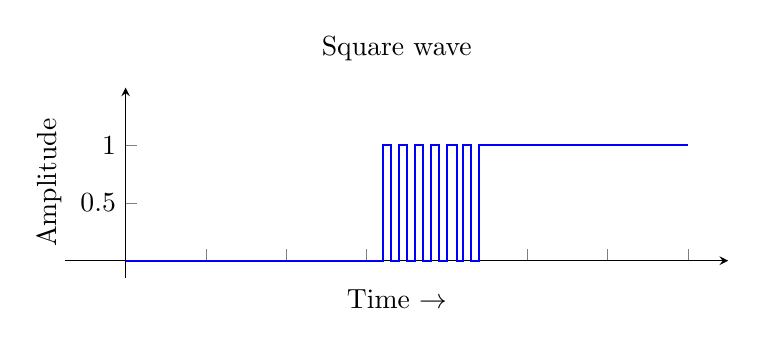
\begin{tikzpicture}
		\begin{axis}[
			width=10cm,
			height=4cm,
			x axis line style={-stealth},
			y axis line style={-stealth},
			title={Square wave},
			xticklabels={},
			ymax = 1.5,xmax=7.5,
			axis lines*=center,
			ytick={0.5,1},
			xlabel={Time $\rightarrow$},
			ylabel={Amplitude},
			xlabel near ticks,
			ylabel near ticks]
			\addplot+[thick,mark=none,const plot]
			coordinates
			{(0,0) (3,0) 
			(3.1,0) (3.2,1) (3.3,0) (3.4,1) (3.5,0) (3.6,1) (3.7,0)
			(3.8,1) (3.9,0) (4.0,1) (4.12,0) (4.2,1) (4.3,0) (4.4,0) (4.4,1) (7,1)
			};
			
			
		\end{axis}
	\end{tikzpicture}
	
\end{document}